\documentclass[aps,prl,twocolumn,floatfix,10pt,amssymb,amsfont,amsmath,superscriptaddress,float,nofootinbib,longbibliography,nobalancelastpage]{revtex4-2}
\usepackage{graphicx} % Required for inserting images
\usepackage[export]{adjustbox}
\usepackage[T3,T1]{fontenc}
\usepackage{braket}
\usepackage{bm}
\DeclareSymbolFont{tipa}{T3}{cmr}{m}{n}
\DeclareMathAccent{\invbreve}{\mathalpha}{tipa}{16}



\begin{document}
\title{Local Hubbard Model Spin Duality}

\begin{abstract}

\end{abstract}
\maketitle

\section{Introduction}
The Hubbard model is a cornerstone of modern condensed matter physics, capturing essential features of strongly correlated electron systems \cite{}. Despite its apparent simplicity, the Hubbard model remains analytically intractable in most regimes \cite{} and is computationally challenging for classical simulations \cite{}. 

Quantum computers offer a promising avenue to overcome these limitations by directly simulating quantum many-body systems \cite{}. However, mapping fermionic degrees of freedom to qubits is a nontrivial task with many subtleties. Conventional fermion-to-qubit mapping schemes 
\cite{Bravyi_2002,Verstraete_2005,Hastings:2014wyq, PhysRevA.94.030301, PhysRevA.95.032332,PhysRevResearch.1.033033, Steudtner_2019, Backens_2019,Jiang_2020, PhysRevB.104.035118,Chiew_2023,PRXQuantum.4.030314,PRXQuantum.4.010326,PhysRevB.109.115149}
 neglect crucial details when implementing periodic boundary conditions. These omissions can lead to unphysical results, as demonstrated in recent work \cite{OBrien:2024tiu}, which highlights the importance of correctly accounting for noncontractible loop operators and their role in determining the physical fermionic boundary conditions.

In this work, we propose a novel fermion-to-qubit mapping tailored to the Hubbard model. Leveraging the flexibility of fermionic tensor networks \cite{}, specifically Projected Entangled Pair Operators (PEPOs) \cite{}, we construct a dual spin representation that respects the model's symmetries and facilitates the use of periodic boundary conditions. This approach addresses the significant finite-size effects encountered in small-scale simulations and ensures that the correct fermionic physics is faithfully reproduced.

Our mapping not only incorporates periodic boundary conditions but also reveals a deeper connection between the fermionic system and its spin dual. By gauging the fermion parity symmetry of the model, our construction introduces both matter and gauge fields in the spin representation, differing from existing mappings that solely produce spins on edges. Furthermore, we explore how the symmetries of the Hubbard model manifest in the spin dual system.

The paper is organized as follows: In Sec. II, we detail our mapping procedure using fermionic tensor networks and demonstrate its application to the Hubbard model. Sec. III discusses the implementation of boundary conditions, emphasizing the necessity of correctly selecting charge sectors for periodic systems. Finally, in Sec. IV, we examine how the Hubbard model's symmetries transform under the mapping and outline the implications for quantum simulation.

\section{Mapping}
Our mapping demonstrates the power of using fermionic tensor networks (PEPOs) to generate fermion-to-qubit mappings (as first introduced by \cite{Shukla:2019ggq}). We rely heavily upon the notation and techniques of \cite{OBrien:2024tiu} to describe our fermionic PEPO. We focus on describing the Hubbard model on a square lattice, but the flexibility of the fermionic PEPO approach allows this to be easily extended to any lattice.

Our fermionic tensor network consists of three tensors: an edge tensor, a 5-leg vertex tensor, and a 3-leg vertex tensor. These are defined as:
\begin{equation}
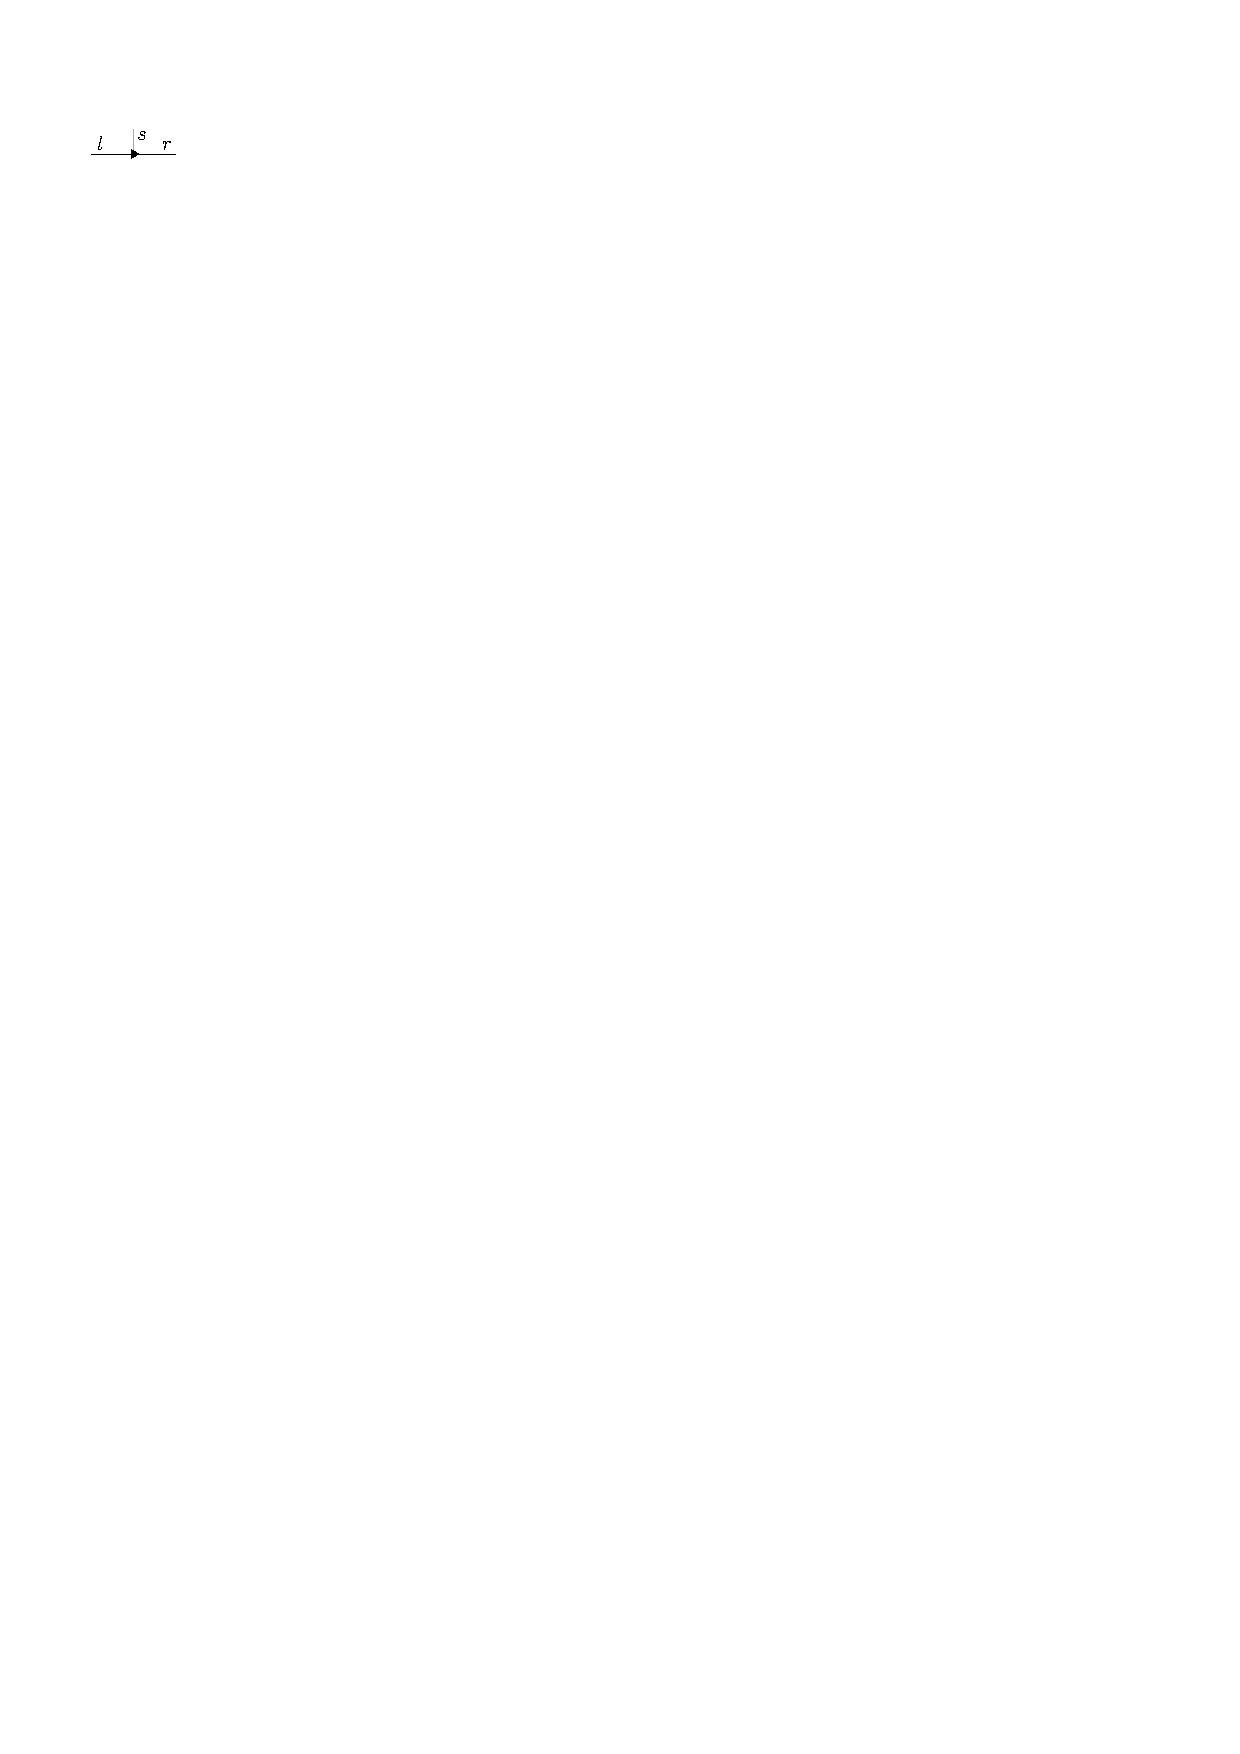
\includegraphics[page=1,valign=c]{Figures.pdf} := \sum_{c} \langle c|_s (c|_l (c|_r,
\end{equation}
\begin{equation}
    \includegraphics[page=2,valign=c]{Figures.pdf} := \hspace{-1em} \sum_{\substack{\{a_i\} \\ \sum_i a_i = 0\, (\text{mod}\, 2)}} \hspace{-1em} |a_4)|a_3)|a_2) |a_1) |a_0),
\end{equation}
\begin{equation}
    \includegraphics[page=3,valign=c]{Figures.pdf}:= \hspace{-1em} \sum_{\substack{\{a_i\} \\ \sum_i a_i = 0\, (\text{mod}\, 2)}} \hspace{-1em} |a_2) |a_1) |a_0).
\end{equation}

By contracting these tensors into the following PEPO, we describe a transformation from physical fermionic degrees of freedom (wiggly lines with spins labeled by arrows) to physical spin degrees of freedom (grey lines). 
\begin{equation*}
    \includegraphics[page=4]{Figures.pdf}
\end{equation*}
It is interesting to note that we have mapped from fermions on vertices to spins on edges \textbf{and} vertices. This is unlike existing fermion-to-qubit mappings which map fermions on vertices to spins on edges. We consider this to imply the joint $\mathbb{Z}_2$ gauging of the fermionic parity of both fermion species produces both matter and gauge fields.

The easiest way to follow the action of this mapping is to consider the transformation of fermionic operators into spin operators. This is done by utilising the symmetries of the tensors as outlined in \cite{OBrien:2024tiu}. We follow their convention and consider the transformation of majorana fermionic operators defined as $\invbreve X_{i,\sigma} = c^{\dagger}_{i,\sigma}+ c_{i,\sigma}$ and $\invbreve Z_{i,\sigma} = 1- 2c^{\dagger}_{i,\sigma}c_{i,\sigma}$:
\begin{equation}
    \includegraphics[page=5,valign=c]{Figures.pdf} = \includegraphics[page=6,valign=c]{Figures.pdf},
\end{equation}
\begin{equation}
    \includegraphics[page=7,valign=c]{Figures.pdf} = \includegraphics[page=8,valign=c]{Figures.pdf},
\end{equation}
\begin{equation}
    \includegraphics[page=9,valign=c]{Figures.pdf} = -\includegraphics[page=20,valign=c]{Figures.pdf},
\end{equation}
\begin{equation}
    \includegraphics[page=10,valign=c]{Figures.pdf} = \includegraphics[page=12,valign=c]{Figures.pdf},
\end{equation}
\begin{equation}
    \includegraphics[page=13,valign=c]{Figures.pdf} = \includegraphics[page=17,valign=c]{Figures.pdf},
\end{equation}
\begin{equation}
    \includegraphics[page=14,valign=c]{Figures.pdf} = -\includegraphics[page=16,valign=c]{Figures.pdf}.
\end{equation}
We can use this to write the dual spin Hamiltonian of the Hubbard model (in the bulk). The Hubbard Model contains hopping terms and onsite interaction terms:
\begin{equation}
    H = - t\sum_{<i,j>, \sigma}  (c^{\dagger}_{i\sigma}c_{j \sigma} + c^{\dagger}_{j\sigma}c_{i \sigma}) + U \sum_{i} c^{\dagger}_{i \uparrow} c^{\dagger}_{i\downarrow} c_{i \downarrow} c_{i  \uparrow}
\end{equation}

This can be rewritten in terms of majorana fermionic operators:
\begin{multline}
    H = -\frac{t}{2} \sum_{<i,j>, \sigma}  (\invbreve X_{i,\sigma}\invbreve Z_{j,\sigma}\invbreve X_{j,\sigma} + \invbreve X_{j,\sigma}\invbreve Z_{i,\sigma}\invbreve X_{i,\sigma}) +\\ \frac{U}{4} \sum_{i} (1-\invbreve Z_{i,\uparrow}-\invbreve Z_{i,\downarrow}+\invbreve Z_{i,\uparrow}\invbreve Z_{i,\downarrow})
\end{multline}
Therefore, the dual spin Hamiltonian (in the bulk) is given by:
\begin{align}
\label{eq:spin_hubbard}
\begin{split}
    H_{hub} = -\frac{t}{2} \sum \left(-\includegraphics[page=15,valign=c]{Figures.pdf} &+ \includegraphics[page=17,valign=c]{Figures.pdf}\right. \\
    -\includegraphics[page=16,valign=c]{Figures.pdf} &+\includegraphics[page=18,valign=c]{Figures.pdf}\\
    +\includegraphics[page=11,valign=c]{Figures.pdf} &- \includegraphics[page=20,valign=c]{Figures.pdf}\\
    +\includegraphics[page=12,valign=c]{Figures.pdf} &-  \left. \includegraphics[page=19,valign=c]{Figures.pdf}\right) \\
    +\frac{U}{4}\sum \left(1- \includegraphics[page=6,valign=c]{Figures.pdf} &- \includegraphics[page=8,valign=c]{Figures.pdf}\right. \\
    &+\left.\includegraphics[page=21,valign=c]{Figures.pdf}\right). \\
    \end{split}
\end{align}
\section{Boundary conditions}
Now we have the mapping in the bulk we can simulate the Hubbard model on a quantum computer with open boundary conditions. However, for small simulations (e.g. 5x5 sites) the boundary will make up a large proportion of the total model (e.g. 16 out of 25). Therefore, finite size effects will have an enormous impact. Hence it is highly desirable to use periodic boundary conditions which would help negate these effects.

We do not yet know a local spin representation for the fermionic operators that act across the boundary. One could represent these operators with a string of spins that transverse the whole bulk to connect the boundaries, but this will obviously lead to inefficient simulation. 

It is important to note that the naive approach to extending this mapping (and all other fermion-to-qubit mapping schemes) to periodic boundary conditions is flawed. Every `local' fermion-to-qubit mapping scheme is only a valid spin representation of the fermionic creation and annhilation operators on the -1 joint eigenspace of the spin gauge conditions (stabilisers):
\begin{equation}
    \includegraphics[page=24,valign=c]{Figures.pdf}.
\end{equation}
When we attempt to project onto this space with periodic boundary conditions we will find there is remaining degeneracy, as the local gauge conditions (stabilisers) are no longer independent. Therefore, unless we also project onto the correct eigenspace of the non-contractible gauge conditions we will fail to capture the correct physics. 

\cite{OBrien:2024tiu} demonstrated the mapping between eigenspaces of these non-contractible gauge conditions (charge sectors) and the fermionic boundary conditions. This correspondence was shown to depend upon the fermionic parity sector being mapped. Using these techniques we can pick the correct charge sector and boundary conditions of the dual spin model to correspond to particular fermionic boundary conditions and parity sector.

To exemplify why this is so important let us consider a simple 1D spin duality \cite{OBrien:2024tiu}.
\begin{equation}
    H = \sum_{i=0}^{N-1} \invbreve X_{i}\invbreve Z_{i+1}\invbreve X_{i+1} + \invbreve X_{N}\invbreve Z_{0}\invbreve X_{0}
\end{equation}
\begin{equation}
    \tilde H = \sum_{i=0}^{N-1}Z_{i-\frac{1}{2}}Z_{i+\frac{1}{2}}X_{i+\frac{1}{2}} + Z_{N-\frac{1}{2}}Z_{\frac{1}{2}}X_{\frac{1}{2}}
\end{equation}
$\tilde H$ will only be a valid representation of $H$ (on the even-parity fermionic sector) in the $-1$ eigenspace of the $\prod_i X_i$ operator. If we had mistakenly restricted to the $+1$ eigenspace of $\prod_i X_i$, then in order to map to a valid even-parity fermionic state we must use a fermionic MPO with a $\invbreve Z$ boundary condition, which would instead map $\tilde{H}$ to $H'$:
\begin{equation}
    H = \sum_{i=0}^{N-1} \invbreve X_{i}\invbreve Z_{i+1}\invbreve X_{i+1} - \invbreve X_{N}\invbreve Z_{0}\invbreve X_{0}
\end{equation}

For the Hubbard Model we will only consider perioidic boundary conditions for simplicity. However, it remains essential to consider the even and odd fermion parity sectors separately.

For the even parity sector (with periodic fermionic boundary conditions) we have trivial spin boundary conditions ($H_{even} =H_{hub}$), however we do need to restrict our spin system to the joint -1 eigenspace of the following charge sectors:
\begin{equation}
    \includegraphics[page=22,valign=c]{Figures.pdf},
\end{equation}
\begin{equation}
    \includegraphics[page=23,valign=c]{Figures.pdf}.
\end{equation}

However, for the odd parity sector (with periodic fermionic boundary conditions) we instead restrict to the joint +1 eigenspace of these charge sectors, but we now have a twisted spin boundary condition. All the terms in the spin Hamiltonian are as described in \eqref{eq:spin_hubbard} with the signs of some operators flipped on one boundary site $(\circ)$:
\begin{align}
\begin{split}
   H_{odd} = H_{hub}-t \left(-\includegraphics[page=25,valign=c]{Figures.pdf} &+ \includegraphics[page=27,valign=c]{Figures.pdf} -\includegraphics[page=39,valign=c]{Figures.pdf}\right. \\
    -\includegraphics[page=26,valign=c]{Figures.pdf} + \includegraphics[page=28,valign=c]{Figures.pdf} &-\includegraphics[page=40,valign=c]{Figures.pdf}\\
     +\includegraphics[page=29,valign=c]{Figures.pdf}&+\left.\includegraphics[page=30,valign=c]{Figures.pdf} \right)\\
    +\frac{U}{2}\left( \includegraphics[page=31,valign=c]{Figures.pdf}\right.&-\left.\includegraphics[page=32,valign=c]{Figures.pdf} \right) \\
    \end{split}
\end{align}

\section{Symmetries}
The Hubbard Model contains more symmetries than just the fermion parity symmetry we gauged when moving to our dual model. Therefore, it is interesting to understand how the generators of these symmetries are transformed by the mapping.

The Hubbard Model conserves fermion particle number $\invbreve N = \sum_{i,\sigma} c^{\dagger}_{i \sigma} c_{i \sigma}$ giving it the $U(1)$ symmetry:
\begin{equation}
    \invbreve U = e^{i\theta \invbreve N}.
\end{equation}
The mapping of this symmetry depends upon the fermionic parity sector we wish to map. For the even parity sector $\invbreve N = \sum_{i,\sigma} \frac{1-\invbreve Z_{i,\sigma}}{2}$ is mapped to:
\begin{equation}
    N_{even} = \sum \left(1 - \frac{1}{2}\includegraphics[page=6,valign=c]{Figures.pdf} - \frac{1}{2}\includegraphics[page=8,valign=c]{Figures.pdf}\right),
\end{equation}
and that the new $U(1)$ symmetry is given by $U_{even} = e^{i\theta N_{even}}$. Whereas for the odd fermionic parity sector, at the boundary there is sign flip on one boundary site $(\circ)$:
\begin{equation}
    N_{odd} = N_{even} + \includegraphics[page=31,valign=c]{Figures.pdf},
\end{equation}
with the $U(1)$ symmetry given by $U_{odd} = e^{i\theta N_{odd}}$.


The Hubbard Model also has an $SU(2)$ symmetry due to the freedom to reorientate the direction of all the spins. We define global spin operators which each commute with the Hubbard Hamiltonian:
\begin{equation}
    \invbreve{S_x} = \frac{1}{2}\sum_{i} c^{\dagger}_{i \uparrow}c_{i \downarrow} + c^{\dagger}_{i \downarrow}c_{i \uparrow},
\end{equation}
\begin{equation}
    \invbreve{S_y} = \frac{i}{2}\sum_{i} c^{\dagger}_{i \uparrow}c_{i \downarrow} - c^{\dagger}_{i \downarrow}c_{i \uparrow},
\end{equation}
\begin{equation}
    \invbreve{S_z} = \frac{1}{2} \sum_{i} (c^{\dagger}_{i \downarrow} c_{i \downarrow}-c^{\dagger}_{i \uparrow} c_{i \uparrow}).
\end{equation}
Therefore, the $SU(2)$ symmetry is generated by:
\begin{equation}
    \invbreve V = e^{i (\bm n \cdot \invbreve{\bm S})},
\end{equation}
where $\invbreve{\bm S} = (\invbreve{S_x}, \invbreve{S_y}, \invbreve{S_z})$.

Again the mapping will depend upon the fermionic parity sector. For the even sector the generators are mapped to:
\begin{equation}
    {S_{x}^{even}} = \frac{1}{2}\sum\includegraphics[page=35,valign=c]{Figures.pdf}-\includegraphics[page=33,valign=c]{Figures.pdf},
\end{equation}
\begin{equation}
   {S_{y}^{even}} = \frac{1}{2}\sum \includegraphics[page=36,valign=c]{Figures.pdf}-\includegraphics[page=34,valign=c]{Figures.pdf},
\end{equation}
\begin{equation}
    {S_{z}^{even}} = \frac{1}{2} \sum \includegraphics[page=6,valign=c]{Figures.pdf} -\includegraphics[page=8,valign=c]{Figures.pdf} .
\end{equation}
with the $SU(2)$ symmetry given by $V_{even} = e^{i (\bm n \cdot \bm S_{even})}$ where $\bm S_{even} = (S_{x}^{even}, S_{y}^{even}, S_{z}^{even})$.

Whereas for the odd fermionic parity sector the generators are modified by a sign flip on one boundary site ($\circ$):
\begin{equation}
    {S_{x}^{odd}} = {S_{x}^{even}} + 
    \includegraphics[page=37,valign=c]{Figures.pdf},
\end{equation}
\begin{equation}
   {S_{y}^{odd}} = {S_{y}^{even}} + \includegraphics[page=38,valign=c]{Figures.pdf},
\end{equation}
\begin{equation}
    {S_{z}^{odd}} = {S_{z}^{even}} + \includegraphics[page=32,valign=c]{Figures.pdf} .
\end{equation}
\section{Conclusion}
In this work, we introduced a novel fermion-to-qubit mapping tailored to the Hubbard model. By leveraging the power of fermionic tensor networks, specifically Projected Entangled Pair Operators (PEPOs), we constructed a dual spin representation that faithfully captures the symmetries and physics of the Hubbard model while accommodating periodic boundary conditions.

We demonstrated the application of this mapping to the Hubbard model on a square lattice, highlighting how the transformation of fermionic operators into spin operators results in a dual spin Hamiltonian that respects the model's inherent symmetries. Furthermore, we addressed the crucial role of charge sectors and non-contractible loop operators in determining the physical boundary conditions, ensuring that our mapping remains valid across different fermionic parity sectors.

While this paper focused on the square lattice for its simplicity, the proposed mapping is equally applicable to other lattice geometries, such as the hexagonal lattice. Applying our method to the hexagonal lattice would result in a more efficient fermion-to-qubit ratio of 1.25 and a reduced maximum Pauli weight of the dual spin Hamiltonian, which would further optimize quantum simulations. However, we chose the square lattice to facilitate a more straightforward demonstration of the mapping's principles and implications. Future work could extend this framework to other lattice geometries to harness these advantages and further refine the mapping for practical quantum computation.

Our results provide a robust framework for simulating strongly correlated electron systems on quantum hardware, offering both conceptual insights and practical tools for advancing quantum simulations of the Hubbard model and beyond.
\bibliography{references}
\end{document}
